\begin{center}
  \textsf{Листок 4.}
\end{center}
\vspace{0.01mm}
\nopagebreak[2]
\taskpic{К свободному концу нити, прикреплённой к стене и перекинутой
  через блок, подвешен груз. Блок закреплён на бруске массы $m_0$,
  который может скользить по горизонтальной плоскости без трения. В
  начальный момент нить с грузом отклоняют от вертикального положения
  на угол $\alpha$ и затем отпускают. Определите ускорение бруска, если
  угол, образованный нитью с вертикалью, не меняется при движении
  системы. Чему равна масса груза.  }{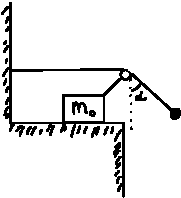
\includegraphics[width=4cm]{p09_13.pdf}}

\task{Где находится центр масс: однородного прута, согнутого
  посередине под прямым углом; однородной треугольной пластинки;
  гардеробного номерка в виде диска с круглым отверстием.  }

\taskpic{ Обезьяна массы $m$ уравновешена противовесом на блоке $А$. Блок $А$
  уравновешен грузом массы $2m$ на блоке $В$. Система неподвижна. Как
  будет двигаться груз, если обезьяна начнёт равномерно выбирать
  верёвку со скоростью $V$ относительно себя? Массой блоков и трением
  пренебречь.}{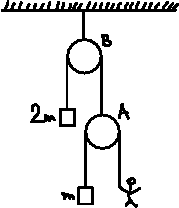
\includegraphics[width=4cm]{p09_15.pdf}}

\task{ С какой силой давит на землю кобра, когда она, готовясь к
  прыжку, поднимается вертикально вверх с постоянной скоростью $V$?
  Масса змеи $m$, её длина $l$.  }
